\documentclass[11pt,a4paper]{article}
\usepackage[margin=2.2cm]{geometry}
\usepackage{lmodern}
\usepackage[T1]{fontenc}
\usepackage{amsmath,amssymb}
\usepackage{graphicx}
\usepackage{booktabs}
\usepackage{caption}
\usepackage{subcaption}
\usepackage{xcolor}
\usepackage[numbers,sort&compress]{natbib}
\usepackage[colorlinks=true,linkcolor=teal,citecolor=teal,urlcolor=teal]{hyperref}
\graphicspath{{../results/figures/}}
% generated by scripts/make_paper_numbers.py, do not edit
\newcommand{\AccCFull}{93.4\%}
\newcommand{\AccLoCFull}{92.1\%}
\newcommand{\AccHiCFull}{94.5\%}
\newcommand{\FOneCFull}{0.933}
\newcommand{\NCFull}{1,600}
\newcommand{\AccCDedup}{93.1\%}
\newcommand{\AccLoCDedup}{91.8\%}
\newcommand{\AccHiCDedup}{94.5\%}
\newcommand{\FOneCDedup}{0.926}
\newcommand{\NCDedup}{1,347}
\newcommand{\AccCDup}{92.5\%}
\newcommand{\AccLoCDup}{90.0\%}
\newcommand{\AccHiCDup}{95.2\%}
\newcommand{\FOneCDup}{0.652}
\newcommand{\NCDup}{441}
\newcommand{\AccCNoDup}{92.7\%}
\newcommand{\AccLoCNoDup}{90.8\%}
\newcommand{\AccHiCNoDup}{94.3\%}
\newcommand{\FOneCNoDup}{0.864}
\newcommand{\NCNoDup}{980}
\newcommand{\AUCC}{0.989}
\newcommand{\ECERawC}{0.054}
\newcommand{\ECECalC}{0.036}
\newcommand{\TempC}{1.84}
\newcommand{\ThrC}{0.67}
\newcommand{\ValAccC}{98.6\%}
\newcommand{\ValCovC}{98.5\%}
\newcommand{\ValRetC}{99.1\%}
\newcommand{\UncRateC}{3.8\%}
\newcommand{\AccConfC}{95.3\%}
\newcommand{\AccUncC}{44.3\%}
\newcommand{\RecCGlioma}{84.0\%}
\newcommand{\PrecCGlioma}{99.7\%}
\newcommand{\RecCMeningioma}{89.8\%}
\newcommand{\PrecCMeningioma}{93.7\%}
\newcommand{\RecCNotumor}{100.0\%}
\newcommand{\PrecCNotumor}{85.7\%}
\newcommand{\RecCPituitary}{99.8\%}
\newcommand{\PrecCPituitary}{96.6\%}
\newcommand{\GliToNoC}{39}
\newcommand{\GliToMenC}{23}
\newcommand{\MenToNoC}{28}
\newcommand{\MenToPitC}{12}
\newcommand{\DNImages}{7,200}
\newcommand{\DNUniqueMd5}{7,013}
\newcommand{\DExactDuplicateFiles}{340}
\newcommand{\DStrictPairs}{3,484}
\newcommand{\DStrictCrossSplitPairs}{1,270}
\newcommand{\DLinkedPairs}{5,962}
\newcommand{\DLinkedCrossSplitPairs}{2,158}
\newcommand{\DGroups}{5,215}
\newcommand{\DTestImgWithTrainDupStrict}{441}
\newcommand{\DTestImgWithTrainDupLinked}{620}
\newcommand{\DTrainImgRemovedCrossSplit}{1,198}
\newcommand{\DImgInLabelConflictGroups}{13}
\newcommand{\DTestDedupReps}{1,347}
\newcommand{\SubTrain}{3,739}
\newcommand{\SubVal}{663}
\newcommand{\SubTest}{1,600}
\newcommand{\SubExcluded}{1,198}
\newcommand{\StrictDupGlioma}{9}
\newcommand{\ExclGlioma}{58}
\newcommand{\TrainGlioma}{1140}
\newcommand{\StrictDupMeningioma}{105}
\newcommand{\ExclMeningioma}{128}
\newcommand{\TrainMeningioma}{1081}
\newcommand{\StrictDupNotumor}{327}
\newcommand{\ExclNotumor}{836}
\newcommand{\TrainNotumor}{478}
\newcommand{\StrictDupPituitary}{0}
\newcommand{\ExclPituitary}{176}
\newcommand{\TrainPituitary}{1040}
\newcommand{\StrictDupPct}{27.6\%}
\newcommand{\LinkedDupPct}{38.8\%}
\newcommand{\OnnxMB}{16.0}
\newcommand{\OnnxLogitDiff}{3.5e-04}
\newcommand{\CamDiff}{7.3e-06}
\newcommand{\BestEpochC}{12}
\newcommand{\EpochSecC}{125}
\newcommand{\BestEpochN}{1}
\newcommand{\ValAccHistN}{91.0\%}

\hypersetup{pdftitle={Leakage-Aware Brain Tumour MRI Classification with Calibrated, Explainable EfficientNet-B0},
  pdfauthor={Rishabh Aryan}, pdfsubject={White paper}, pdfkeywords={brain tumour MRI, EfficientNet, data leakage, near-duplicates, Grad-CAM, explainable AI, calibration}}
\captionsetup{font=small,labelfont=bf}

\title{\textbf{Leakage-Aware Brain Tumour MRI Classification\\with a Calibrated, Explainable EfficientNet-B0}\\[4pt]\large A white paper on data hygiene, explanation quality and an in-browser research demo}
\author{Rishabh Aryan\\[2pt]
\small M.Tech (Artificial Intelligence and Data Science), Department of Computer Science and Engineering\\
\small Indian Institute of Information Technology Bhagalpur, Bihar, India}
\date{November 2026}

\begin{document}
\maketitle

\begin{abstract}
\noindent Public brain MRI collections are widely used to benchmark four-way tumour classifiers (glioma, meningioma, pituitary tumour, no tumour), and reported accuracies often approach 99\%. We revisit the popular Kaggle \emph{Brain Tumor MRI Dataset} (version~2, \DNImages{} images) with an emphasis on evaluation hygiene. A perceptual-hash audit shows that, although no file is byte-identical across the official Training and Testing folders, \DTestImgWithTrainDupStrict{} of the 1{,}600 Testing images (\StrictDupPct{}) have a strict near-duplicate in Training, concentrated in the no-tumour class. We remove every Training image linked to a Testing image, split the remainder into train and validation sets by duplicate group, and fine-tune an ImageNet-pretrained EfficientNet-B0 on a CPU. On the full Testing folder the model reaches \AccCFull{} accuracy (95\% bootstrap CI \AccLoCFull{}--\AccHiCFull{}), macro-F1 \FOneCFull{} and macro one-vs-rest ROC-AUC \AUCC{}, while validation accuracy inside the training distribution is \ValAccC{}. Temperature scaling (T~=~\TempC{}) reduces the expected calibration error on Testing from \ECERawC{} to \ECECalC{}, and a confidence threshold chosen on validation flags \UncRateC{} of Testing predictions as uncertain. We compare five attribution methods (Grad-CAM, Grad-CAM++, Integrated Gradients, occlusion and KernelSHAP on superpixels) with the model-parameter randomisation sanity check and deletion/insertion faithfulness metrics. The model, exported to ONNX, runs in the browser with exact Grad-CAM, occlusion and a templated ``why this prediction'' panel that uses only model outputs and measured test statistics. The system is a research and education artefact, not a medical device.
\end{abstract}

\section{Introduction}
Brain tumours are a heterogeneous group of neoplasms whose diagnosis rests on imaging, histology and, since the 2021 WHO classification, molecular markers \citep{louis2021}. Magnetic resonance imaging is the main imaging modality, and automatic slice-level classification of MRI into broad tumour categories has become a standard exercise for transfer learning in medical imaging \citep{deepak2019,swati2019,badza2020}. Much of this work uses small public collections in which several images come from the same patient or the same scan, and in which the provenance of individual images is only partly documented.

Two problems follow. First, when near-identical slices sit on both sides of a train/test split, test accuracy partly measures memorisation rather than generalisation, a form of leakage that has repeatedly inflated results in applied machine learning \citep{kapoor2023,roberts2021}; even curated vision benchmarks contain such near-duplicates \citep{barz2020}. Second, the saliency maps that often accompany these classifiers are rarely tested: they can look plausible while being insensitive to the model's parameters \citep{adebayo2018}, and in medical images they frequently fail to localise pathology \citep{arun2021,saporta2022}.

This white paper documents a small, fully reproducible project that tries to address both. Our contributions are:
\begin{enumerate}
\item an audit of exact and near-duplicate images in version~2 of the Kaggle Brain Tumor MRI Dataset \citep{nickparvar2021}, with all hashes, pairs and split files released for review;
\item a leakage-aware split and an EfficientNet-B0 \citep{tan2019} baseline trained on a CPU, reported with confidence intervals, per-class metrics, ROC-AUC, calibration and an explicit uncertainty threshold, and compared with a naive split of the same data;
\item a comparison of five attribution methods with sanity checks and faithfulness metrics; and
\item an in-browser demonstrator that reproduces the PyTorch probabilities, computes Grad-CAM exactly from ONNX outputs, and explains each prediction using only measured quantities.
\end{enumerate}

\section{Related work}
\paragraph{Brain tumour classification.} \citet{cheng2015} released the figshare T1-weighted contrast-enhanced collection (glioma, meningioma, pituitary tumour) and classified tumour regions with handcrafted features after region augmentation and partitioning. \citet{deepak2019} and \citet{swati2019} showed that features from ImageNet-pretrained networks \citep{deng2009}, fine-tuned block-wise, reach high accuracy on the same data, and \citet{badza2020} reported a compact CNN evaluated with patient-wise and record-wise cross-validation, noting the gap between the two. The Kaggle dataset used here merges figshare with the SARTAJ and Br35H collections \citep{nickparvar2021}. Volumetric multi-sequence benchmarks such as BraTS \citep{menze2015} target segmentation of gliomas rather than slice-level type classification.

\paragraph{Leakage and duplicates.} \citet{kapoor2023} catalogue leakage as a main cause of irreproducible machine-learning findings, and \citet{roberts2021} found that most COVID-19 imaging models suffered from data duplication across sources and splits. \citet{barz2020} purged near-duplicates from CIFAR and measured the resulting accuracy drop. We use perceptual hashing \citep{zauner2010} combined with pixel correlation to find such pairs.

\paragraph{Explanations and their evaluation.} Occlusion sensitivity \citep{zeiler2014}, Grad-CAM \citep{selvaraju2017} and Grad-CAM++ \citep{chattopadhay2018}, Integrated Gradients \citep{sundararajan2017}, LIME \citep{ribeiro2016} and SHAP \citep{lundberg2017} are common post-hoc attribution methods. \citet{adebayo2018} proposed the model-parameter randomisation test, and \citet{petsiuk2018} introduced the deletion and insertion metrics. Benchmarks in radiology report that saliency maps often fall short of localisation targets \citep{arun2021,saporta2022}. Calibration of modern networks and temperature scaling are due to \citet{guo2017}.

\section{Data and duplicate audit}
\subsection{Dataset}
Version~2 of the Brain Tumor MRI Dataset (13 February 2026, CC BY 4.0) holds \DNImages{} 2-D slices in a \texttt{Training} folder (1{,}400 per class) and a \texttt{Testing} folder (400 per class). According to its description, glioma, meningioma and pituitary images come from figshare \citep{cheng2015} and SARTAJ, no-tumour images come from Br35H, and version~2 removed duplicates and eliminated train/test overlap. Images vary in size (most are $512\times512$) and in sequence and orientation (axial, coronal and sagittal; T1, T1 with contrast, T2 and FLAIR); no patient identifiers are provided. We download it with \texttt{kagglehub} and never redistribute it, apart from eight resized sample slices in the demo, as the licence allows with attribution.

\subsection{Audit method}
For each image we compute the MD5 of the file, a 64-bit DCT perceptual hash (pHash, \texttt{imagehash}) of the greyscale image and a $64\times64$ zero-padded thumbnail. For every pair within a Hamming distance of 10 we compute the Pearson correlation of the thumbnails. Visual inspection of random pairs at each distance showed that pHash alone is too coarse for MRI (many different slices of similar anatomy sit 4--6 bits apart), so we define:
\begin{itemize}
\item \textbf{strict near-duplicate}: identical MD5, or Hamming distance $\le 2$ and correlation $\ge 0.98$ (in our inspection, the same image re-encoded or resized);
\item \textbf{linked}: identical MD5, or Hamming distance $\le 6$ and correlation $\ge 0.95$ (also catches near-identical neighbouring slices of the same scan).
\end{itemize}
Connected components of linked images form \emph{groups}. Thresholds were fixed by inspection before any model was trained; the full candidate-pair list (Hamming $\le 10$) is released so that others can apply different thresholds.

\subsection{Findings}
There are \DExactDuplicateFiles{} files involved in exact duplication (\DNUniqueMd5{} unique MD5 values), none of them across folders, which agrees with the dataset description. Near-duplicates, however, are common: we find \DStrictPairs{} strict pairs, \DStrictCrossSplitPairs{} of them across the Training/Testing boundary, and \DLinkedPairs{} linked pairs (\DLinkedCrossSplitPairs{} across). \DTestImgWithTrainDupStrict{} Testing images (\StrictDupPct{}) have a strict near-duplicate in Training and \DTestImgWithTrainDupLinked{} (\LinkedDupPct{}) are linked to one. The overlap is class-dependent: strict cross-split duplicates affect \StrictDupNotumor{} no-tumour, \StrictDupMeningioma{} meningioma, \StrictDupGlioma{} glioma and \StrictDupPituitary{} pituitary Testing images. \DImgInLabelConflictGroups{} images belong to groups that carry more than one class label. Figure~\ref{fig:dedup} shows examples.

\begin{figure}[t]
\centering
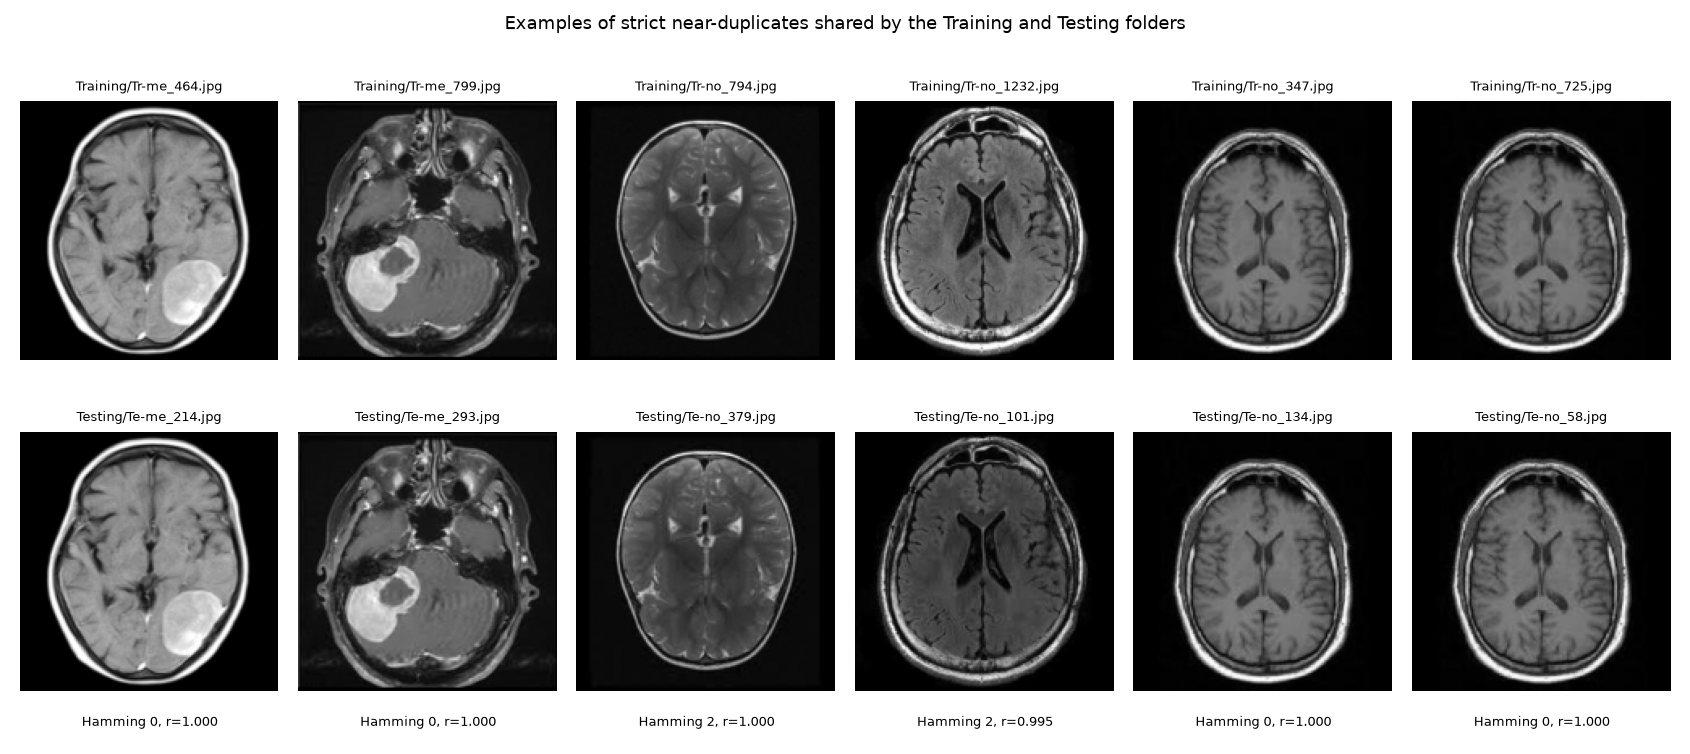
\includegraphics[width=\linewidth]{dedup_examples.png}
\caption{Strict near-duplicates shared by the Training and Testing folders (top: Training file, bottom: matching Testing file, with pHash Hamming distance and thumbnail correlation).}
\label{fig:dedup}
\end{figure}

\subsection{Leakage-aware split}
We remove from the training pool every Training image whose group contains a Testing image (\DTrainImgRemovedCrossSplit{} images) and every image in a label-conflict group, then assign whole groups to validation (about 15\% per class, seeded) and the rest to training. This leaves \SubTrain{} training and \SubVal{} validation images, and keeps the official \SubTest{} Testing images untouched, so the test set is directly comparable with other work while no linked image of it is seen in training. The removal is very uneven (Figure~\ref{fig:removed}): \ExclNotumor{} of the 1{,}400 no-tumour Training images are linked to Testing images, leaving only \TrainNotumor{} for training. We also report results on the Testing folder reduced to one image per group (\NCDedup{} images).

\begin{figure}[t]
\centering
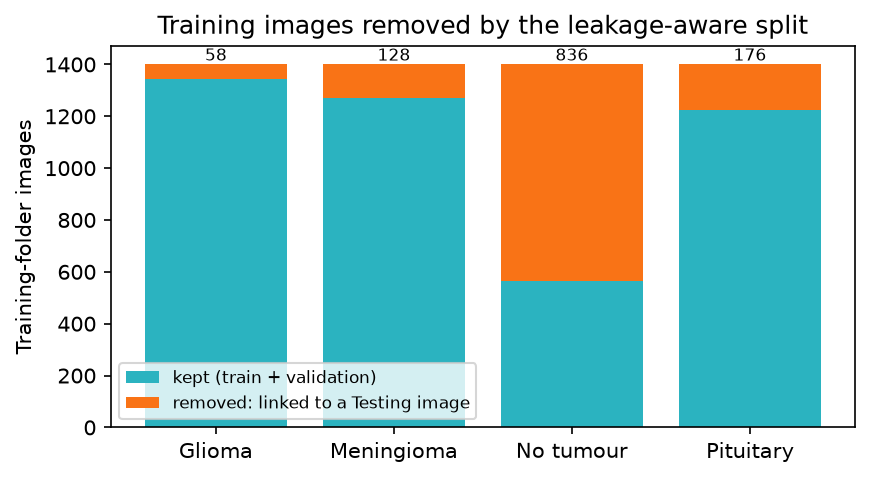
\includegraphics[width=0.62\linewidth]{dedup_per_class.png}
\caption{Training-folder images kept and removed by the leakage-aware split, per class.}
\label{fig:removed}
\end{figure}

\section{Method}
\paragraph{Pre-processing.} Every image is converted to greyscale (ITU-R 601 luma), zero-padded to a square to keep its aspect ratio, resized to $224\times224$ with bilinear filtering, replicated to three channels and normalised with ImageNet statistics. The browser demo implements the same steps.

\paragraph{Model and training.} We fine-tune EfficientNet-B0 \citep{tan2019} pretrained on ImageNet (\texttt{timm} \citep{wightman2019}, \texttt{efficientnet\_b0.ra\_in1k}, 4.0\,M parameters, dropout 0.2) in PyTorch \citep{paszke2019} with AdamW (learning rate $5\times10^{-4}$, weight decay $10^{-4}$), a one-cycle schedule, batch size 32 and 12 epochs. Inverse-frequency class weights compensate for the reduced no-tumour class. Augmentation consists of random resized crops (scale 0.8--1.0), horizontal flips, rotations up to $10^\circ$ with 5\% translation, and brightness/contrast jitter of 0.2. The checkpoint with the best validation macro-F1 is kept (epoch \BestEpochC{}). All random generators are seeded (42). Training ran on an 8-core CPU without a GPU in about \EpochSecC{}\,s per epoch.

\paragraph{Naive comparison.} To measure the effect of the split, we train an identical model on the original Training folder with a random, image-level 15\% validation split and evaluate both models on the same Testing images.

\paragraph{Calibration and uncertainty.} We fit a single temperature on the validation logits by minimising the negative log-likelihood \citep{guo2017}. A prediction is flagged \emph{uncertain} when its calibrated confidence is below a threshold $\tau$, chosen on validation as the smallest value in $\{0.50, 0.51, \dots, 0.99\}$ for which the retained validation predictions reach at least 99\% accuracy. For the leakage-aware model $\tau=\ThrC{}$ (validation coverage \ValCovC{}, retained accuracy \ValRetC{}). The normalised entropy of the calibrated distribution is reported alongside but not thresholded.

\paragraph{Metrics.} We report accuracy and macro-F1 with 95\% bootstrap confidence intervals (1{,}000 resamples), per-class precision, recall and F1, the confusion matrix, one-vs-rest ROC-AUC and the expected calibration error (ECE, 15 bins). All numbers in this paper are generated by scripts from a single saved prediction file per model (\texttt{results/predictions/}); the same file feeds the demo's statistics.

\section{Results}
\subsection{Classification}
Table~\ref{tab:subsets} summarises accuracy on the Testing folder and its subsets, and Table~\ref{tab:perclass} gives per-class results for the leakage-aware model; the confusion matrix and ROC curves are in Figure~\ref{fig:eval}.

\begin{table}[t]
\centering\small
\caption{Accuracy, macro-F1 (95\% bootstrap CIs) and calibrated ECE on the Testing folder and subsets. ``Has strict dup.\ in Training'' = Testing images with a strict near-duplicate in the original Training folder; ``No linked dup.'' = Testing images with no linked image in it. Macro-F1 is omitted for the class-skewed subsets.}
\label{tab:subsets}
\resizebox{\linewidth}{!}{\begin{tabular}{llcccc}
\toprule
Model & Test subset & $n$ & Accuracy [95\% CI] & Macro-F1 [95\% CI] & ECE \\
\midrule
Leakage-aware & Full Testing & 1600 & 0.919 [0.905, 0.932] & 0.919 [0.905, 0.931] & 0.052 \\
Leakage-aware & Testing, one per group & 1342 & 0.919 [0.904, 0.932] & 0.912 [0.895, 0.926] & 0.051 \\
Leakage-aware & Has strict dup.\ in Training & 441 & 0.880 [0.850, 0.912] & -- (class-skewed subset) & 0.092 \\
Leakage-aware & No linked dup.\ in Training & 970 & 0.925 [0.908, 0.940] & -- (class-skewed subset) & 0.046 \\
\midrule
Naive & Full Testing & 1600 & 0.961 [0.951, 0.970] & 0.961 [0.950, 0.970] & 0.022 \\
Naive & Testing, one per group & 1342 & 0.959 [0.948, 0.969] & 0.959 [0.947, 0.969] & 0.023 \\
Naive & Has strict dup.\ in Training & 441 & 0.995 [0.989, 1.000] & -- (class-skewed subset) & 0.005 \\
Naive & No linked dup.\ in Training & 970 & 0.940 [0.926, 0.955] & -- (class-skewed subset) & 0.035 \\
\bottomrule
\end{tabular}}
\end{table}

\begin{table}[t]
\centering\small
\caption{Per-class results of the leakage-aware model on the full Testing folder (n = \NCFull{}).}
\label{tab:perclass}
\begin{tabular}{lcccc}
\toprule
Class & Precision & Recall & F1 & ROC-AUC \\
\midrule
Glioma & 0.968 & 0.843 & 0.901 & 0.968 \\
Meningioma & 0.941 & 0.840 & 0.888 & 0.983 \\
No tumour & 0.816 & 0.998 & 0.898 & 0.996 \\
Pituitary & 0.980 & 0.995 & 0.988 & 1.000 \\
\midrule
Macro average & -- & -- & 0.919 & 0.987 \\
\bottomrule
\end{tabular}
\end{table}

\begin{figure}[t]
\centering
\begin{subfigure}{0.40\linewidth}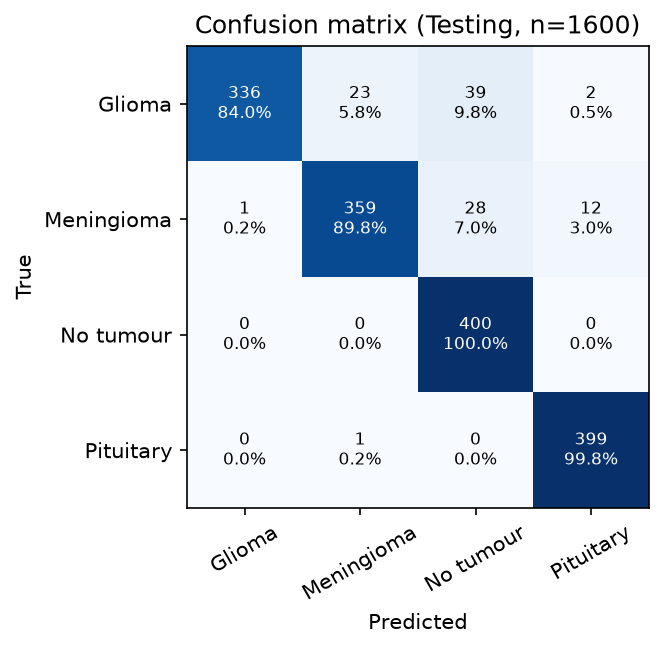
\includegraphics[width=\linewidth]{confusion_matrix.png}\end{subfigure}\hfill
\begin{subfigure}{0.40\linewidth}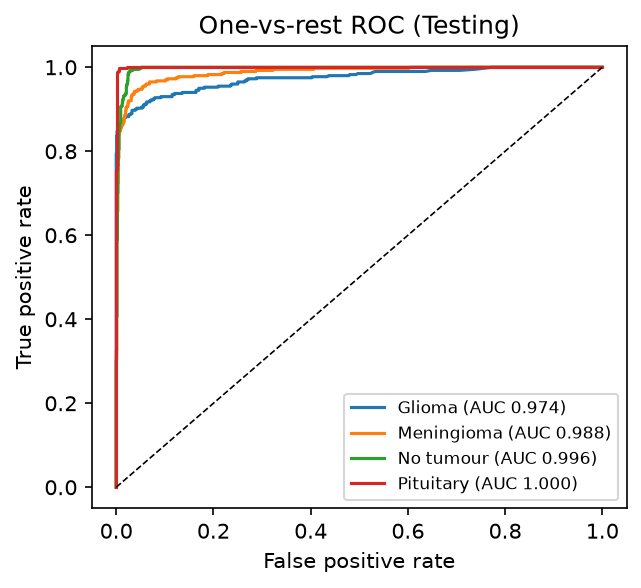
\includegraphics[width=\linewidth]{roc_curves.png}\end{subfigure}
\caption{Leakage-aware model on the Testing folder: confusion matrix (counts and row percentages) and one-vs-rest ROC curves.}
\label{fig:eval}
\end{figure}

The leakage-aware model reaches \AccCFull{} accuracy and macro-F1 \FOneCFull{} on the full Testing folder, and \AccCDedup{} on the one-per-group variant. Errors are not symmetric. Pituitary tumours are almost always recognised (recall \RecCPituitary{}), and every no-tumour image is classified correctly (recall \RecCNotumor{}), but at a cost in no-tumour precision (\PrecCNotumor{}): \GliToNoC{} gliomas and \MenToNoC{} meningiomas are called ``no tumour''. Glioma recall is the lowest (\RecCGlioma{}) although its precision is \PrecCGlioma{}. Missing a tumour is the clinically more serious error, and in this model it is the most frequent one. Validation accuracy (\ValAccC{}) is much higher than test accuracy, which points to a shift between the Training and Testing folders beyond the duplicates we removed (for instance different source collections or acquisition protocols); we could not resolve the source of each image.

%NAIVE_PARAGRAPH%

\subsection{Calibration and uncertainty}
The fitted temperature is \TempC{}, meaning the raw model is over-confident. On Testing, ECE falls from \ECERawC{} to \ECECalC{} (Figure~\ref{fig:calib}). With $\tau=\ThrC{}$, \UncRateC{} of Testing predictions are flagged uncertain; accuracy is \AccConfC{} on the confident ones and \AccUncC{} on the flagged ones. The flag therefore concentrates errors, but most errors on Testing still carry high confidence, so it cannot be treated as a safety net.

\begin{figure}[t]
\centering
\begin{subfigure}{0.40\linewidth}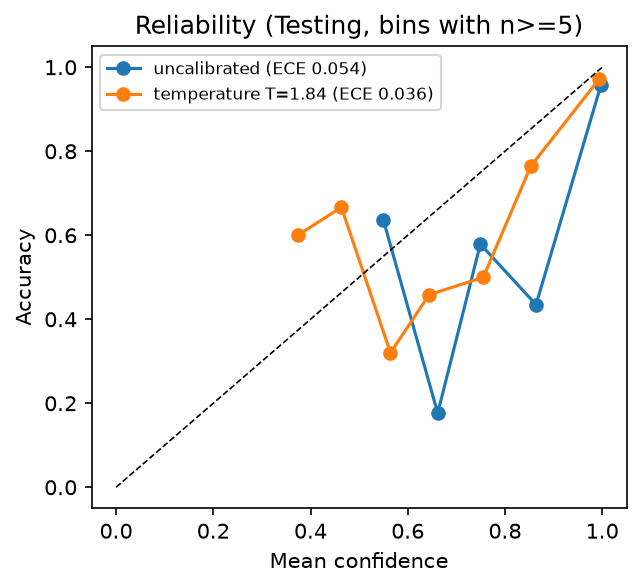
\includegraphics[width=\linewidth]{reliability.png}\end{subfigure}\hfill
\begin{subfigure}{0.56\linewidth}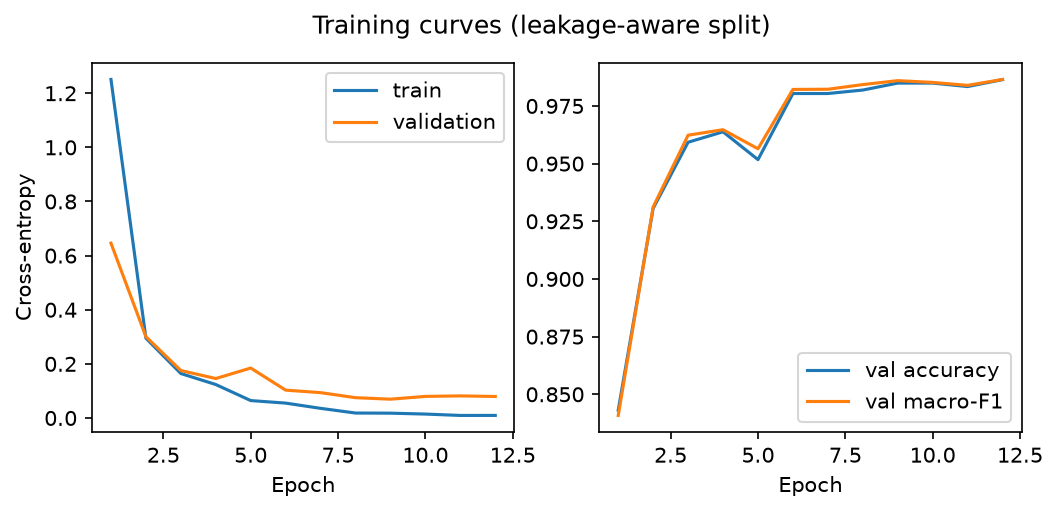
\includegraphics[width=\linewidth]{training_curves_clean.png}\end{subfigure}
\caption{Left: reliability diagram before and after temperature scaling (Testing). Right: training curves of the leakage-aware model.}
\label{fig:calib}
\end{figure}

\section{Explainability}
\subsection{Methods}
All explanations target the predicted class. \textbf{Grad-CAM} weights the final $7\times7\times1280$ feature map by the spatially averaged gradients; because EfficientNet-B0 ends in global average pooling and a linear layer, these weights equal the classifier weights divided by 49, so Grad-CAM coincides with CAM up to a positive scale. We use this to compute Grad-CAM in ONNX without gradients (maximum difference from autograd Grad-CAM after normalisation \CamDiff{}). \textbf{Grad-CAM++} uses the closed-form higher-order weights of \citet{chattopadhay2018}. \textbf{Integrated Gradients} (Captum \citep{kokhlikyan2020}) integrates 32 steps from a black image. \textbf{Occlusion} slides a black $32\times32$ patch with stride 16 and records the drop in the class logit. \textbf{KernelSHAP} \citep{lundberg2017} attributes the class logit to about 64 SLIC superpixels \citep{achanta2012} using 200 coalitions with a black baseline. Signed maps are clipped (occlusion, SHAP) or taken in absolute value (IG), then min--max normalised.

\subsection{Evaluation protocol}
On 100 Testing images (25 per class, seeded) we compute the \emph{deletion} and \emph{insertion} AUC \citep{petsiuk2018}: pixels are removed (set to black) or revealed (from a Gaussian-blurred copy) in 32 equal steps in order of decreasing attribution, and the softmax probability of the target class is integrated over the fraction of pixels. A random attribution serves as baseline. We also measure the share of attribution mass on the bright head region (a crude foreground mask). For the sanity check \citep{adebayo2018} we cumulatively re-initialise the network from the classifier down to the stem on 12 images and compute the Spearman rank correlation between each method's map from the trained and the randomised model; a method that passes should lose correlation as layers are randomised.

\subsection{Results}
Table~\ref{tab:xai} and Figure~\ref{fig:xai} summarise the comparison.

\begin{table}[t]
\centering\small
\caption{Faithfulness (mean $\pm$ s.d.\ over 100 Testing images), attribution mass on the head region, and Spearman correlation with the trained-model map after randomising the classifier only and after randomising the whole network (12 images).}
\label{tab:xai}
\resizebox{\linewidth}{!}{\begin{tabular}{lccccc}
\toprule
Method & Deletion AUC $\downarrow$ & Insertion AUC $\uparrow$ & Mass on head region & $\rho$ after classifier rand. & $\rho$ after full rand. \\
\midrule
Grad-CAM & 0.442 $\pm$ 0.359 & 0.828 $\pm$ 0.215 & 76.3\% & 0.26 & -0.08 \\
Grad-CAM++ & 0.454 $\pm$ 0.346 & 0.823 $\pm$ 0.217 & 81.8\% & 0.91 & 0.05 \\
Integrated Gradients & 0.260 $\pm$ 0.213 & 0.680 $\pm$ 0.259 & 97.7\% & 0.94 & 0.84 \\
Occlusion & 0.387 $\pm$ 0.385 & 0.790 $\pm$ 0.254 & 83.3\% & 0.15 & 0.02 \\
KernelSHAP (SLIC) & 0.419 $\pm$ 0.369 & 0.764 $\pm$ 0.276 & 73.4\% & 0.17 & 0.17 \\
Random baseline & 0.285 $\pm$ 0.106 & 0.424 $\pm$ 0.342 & 57.9\% & -- & -- \\
\bottomrule
\end{tabular}}
\end{table}

%XAI_PARAGRAPH%

\begin{figure}[t]
\centering
\begin{subfigure}{0.62\linewidth}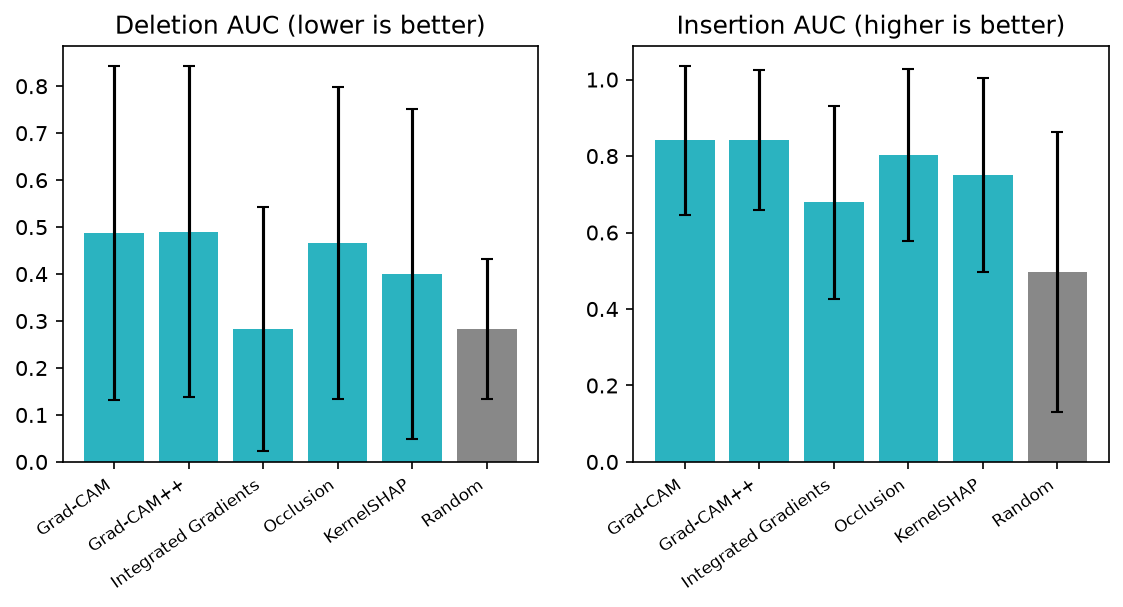
\includegraphics[width=\linewidth]{xai_faithfulness.png}\end{subfigure}\hfill
\begin{subfigure}{0.36\linewidth}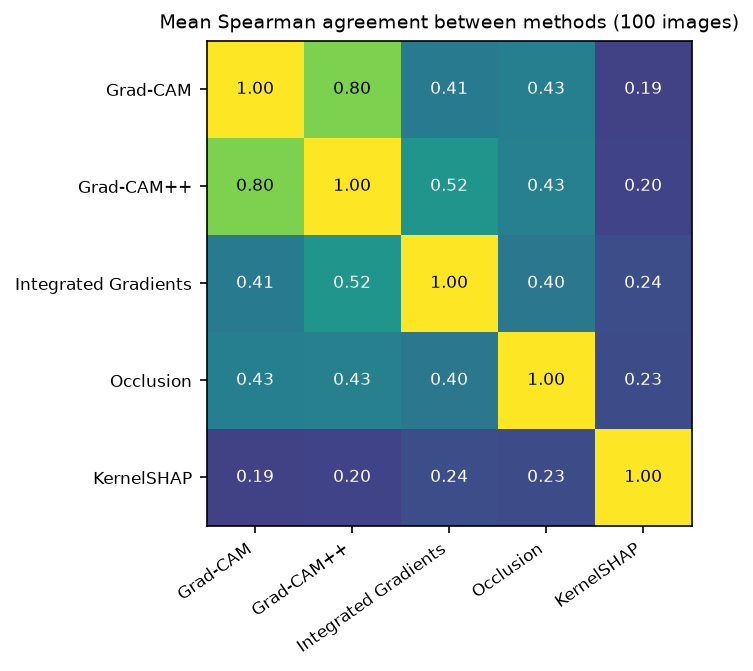
\includegraphics[width=\linewidth]{xai_agreement.png}\end{subfigure}\\[4pt]
\begin{subfigure}{0.6\linewidth}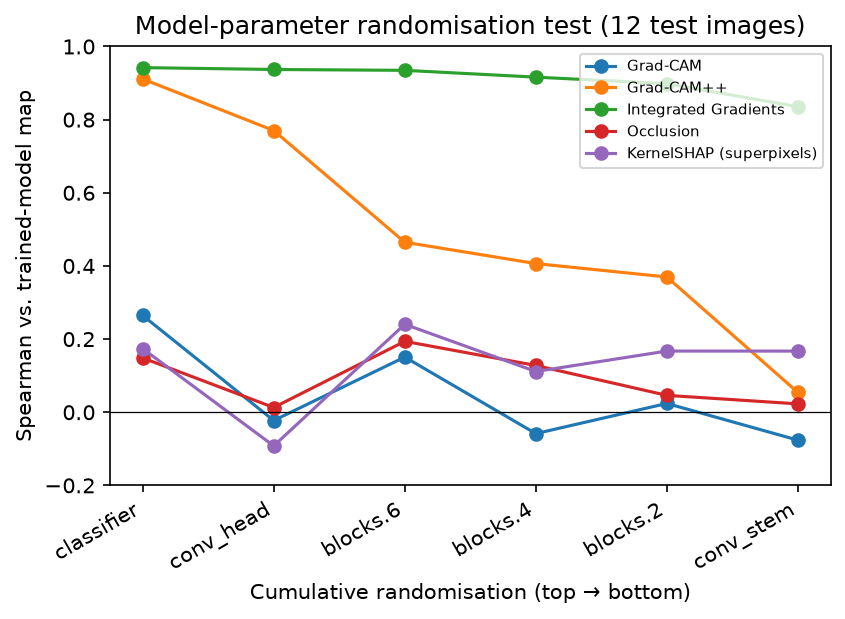
\includegraphics[width=\linewidth]{xai_sanity_check.png}\end{subfigure}
\caption{Top: deletion/insertion AUC per method and mean pairwise Spearman agreement. Bottom: cascading model-parameter randomisation.}
\label{fig:xai}
\end{figure}

\begin{figure}[p]
\centering
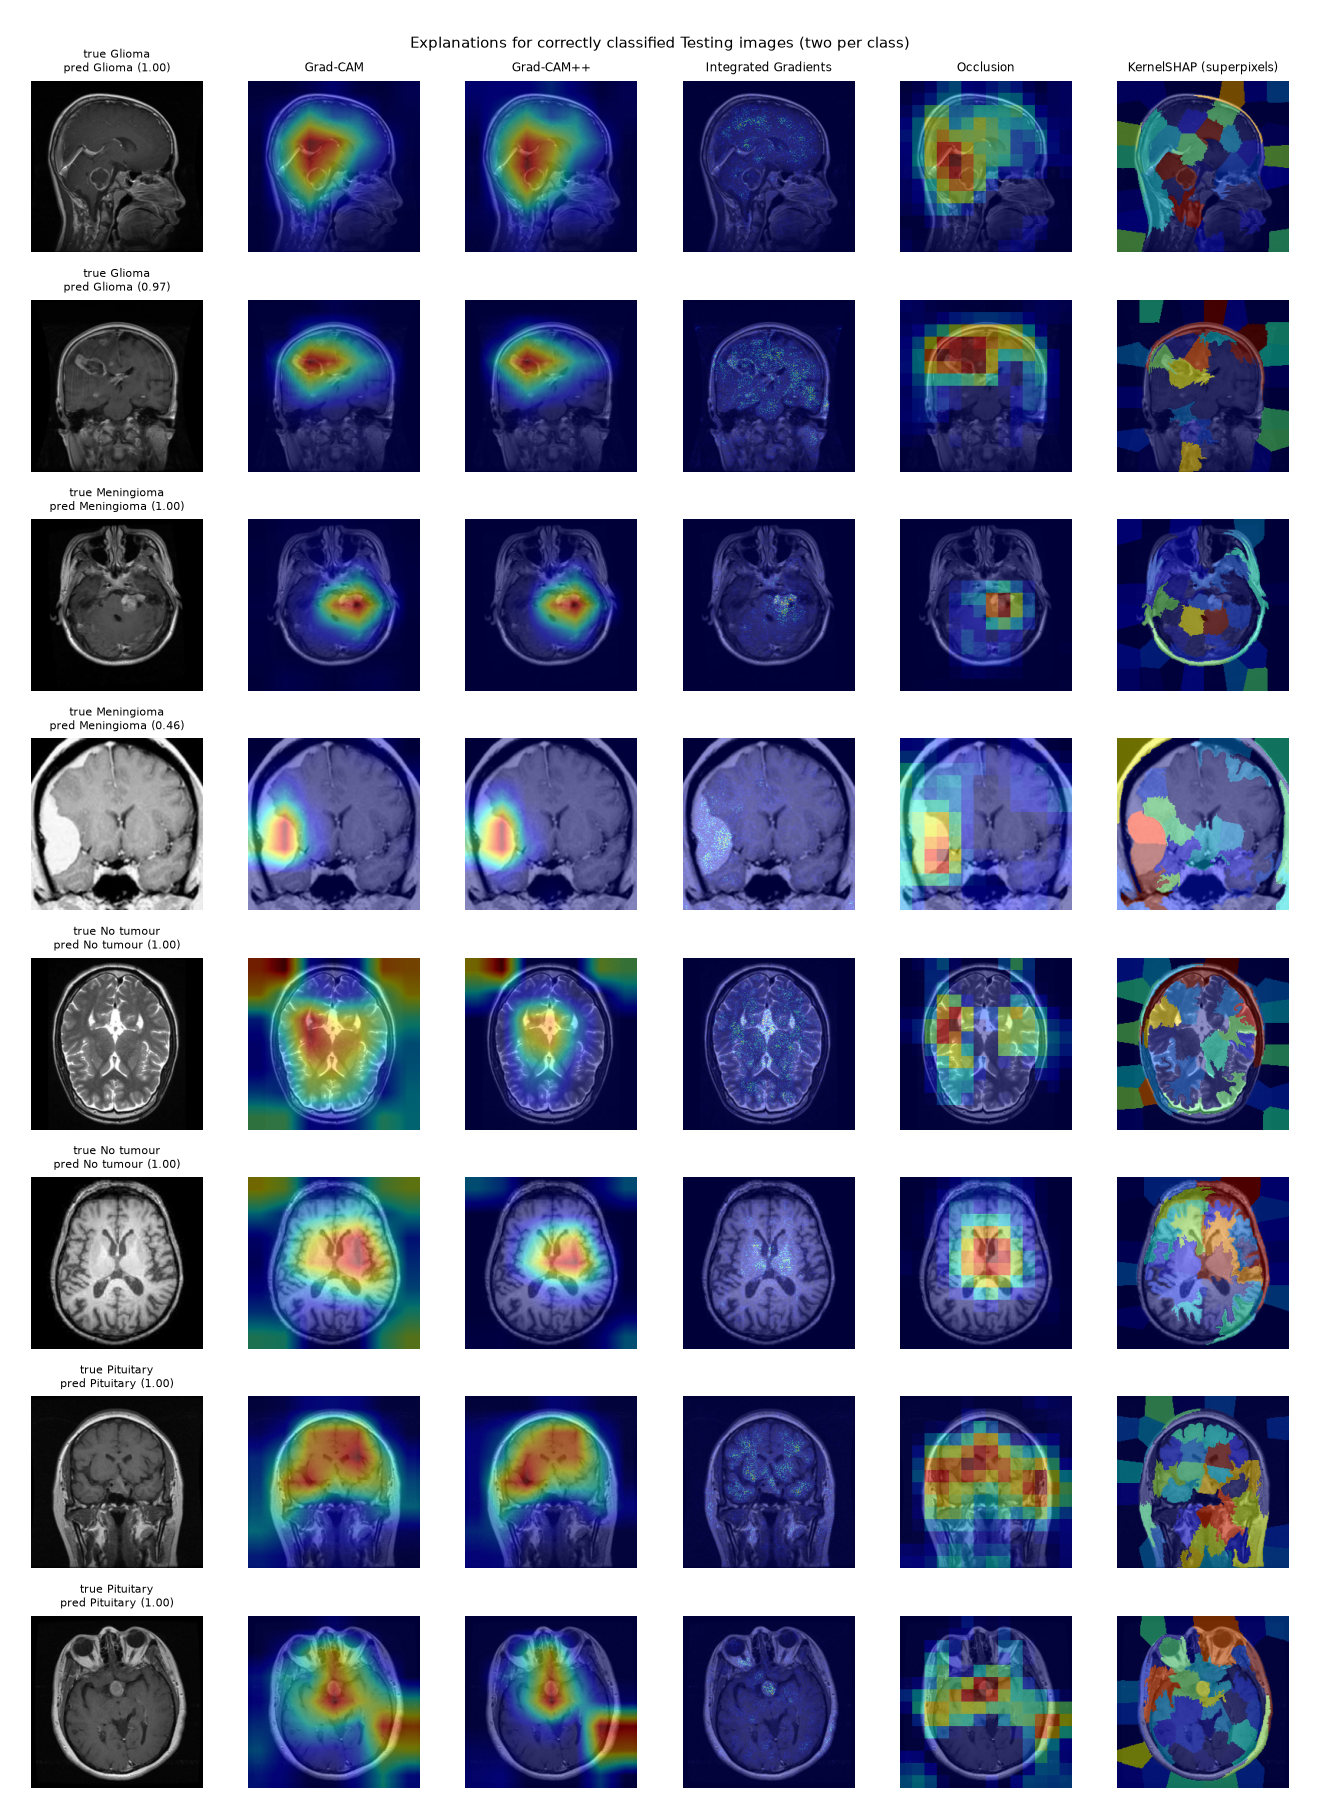
\includegraphics[width=\linewidth]{xai_grid_correct.png}\\[6pt]
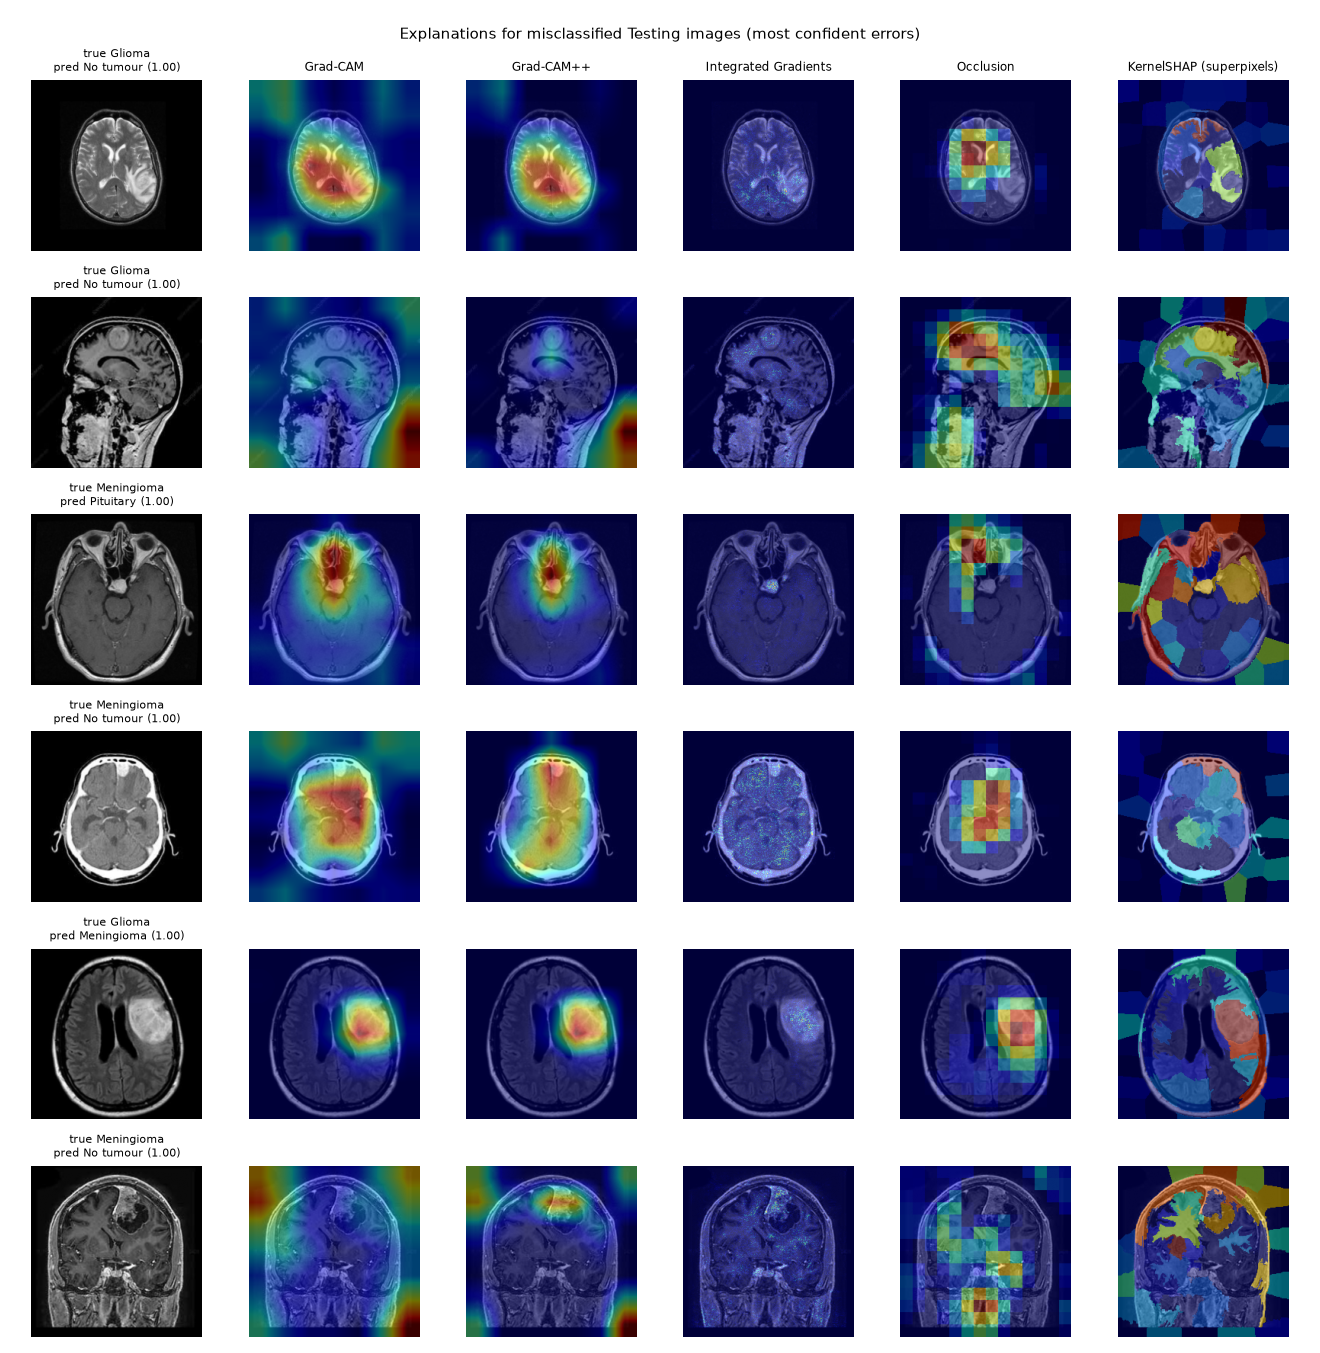
\includegraphics[width=\linewidth]{xai_grid_misclassified.png}
\caption{Explanations for correctly classified Testing images (two per class, top) and for the most confident errors (bottom).}
\label{fig:grids}
\end{figure}

\section{In-browser demonstrator}
The leakage-aware model is exported to ONNX (\OnnxMB{}\,MB) with two outputs, the logits and the four class activation maps, and runs in the browser with ONNX Runtime Web (WebAssembly); the maximum logit difference to PyTorch on 64 Testing images is \OnnxLogitDiff{}. The page replicates the pre-processing, applies the fitted temperature and shows animated class probabilities, a Grad-CAM overlay with an opacity control and an on-demand occlusion map (a $7\times7$ grid of $32$-pixel patches, 49 forward passes). Eight Testing slices (two per class, drawn from images with no linked image in Training) are bundled with their true labels and with precomputed Grad-CAM++, Integrated Gradients and KernelSHAP maps.

A \emph{Why this prediction} panel is generated from templates filled only with measured quantities: the predicted class and calibrated confidence, the margin over the runner-up class, the uncertainty flag ($\tau=\ThrC{}$) and normalised entropy, the share of Grad-CAM mass on the head region and its dominant image quadrant, the rank agreement between methods for the bundled samples, and that class's test precision and recall with its most common confusion, read from the same statistics file as Table~\ref{tab:perclass}. It contains no medical reasoning and is not a diagnosis.

\section{Limitations}
\begin{itemize}
\item \textbf{No patient-level split.} The dataset has no patient identifiers. Our groups capture near-identical images and very similar neighbouring slices, but other slices of the same patient may still occur on both sides of the split, so results may remain optimistic.
\item \textbf{Thresholds by inspection.} The duplicate thresholds were set by looking at examples. Different thresholds change the counts; the released candidate pairs allow re-analysis.
\item \textbf{Source and protocol confounding.} No-tumour images come from a different collection than the tumour classes, so a model can partly learn source characteristics (contrast, resolution, framing) rather than pathology. The gap between validation and test accuracy is consistent with such shifts.
\item \textbf{Slice-level, single-label task.} Real diagnosis uses volumes, several sequences, clinical context and histopathology; this model sees one 2-D slice and four labels and cannot recognise other conditions.
\item \textbf{Single run.} We trained one seed per configuration on a CPU; the confidence intervals reflect test-set sampling only, not training variance.
\item \textbf{Explanations are not localisation.} No tumour masks were used, so we cannot measure whether attributions fall on the lesion; the head-region share is only a sanity proxy.
\end{itemize}

\section{Ethical considerations}
The images are public and de-identified, and we redistribute only eight resized samples under the CC BY 4.0 licence with attribution. A tumour classifier can cause harm if its output is mistaken for a diagnosis: it can miss tumours (the most common error here) and give confident wrong answers. The demonstrator therefore states prominently that it is a research and education tool, not a medical device, processes images locally without uploading them, shows calibrated uncertainty, and builds its rationale only from the model's own outputs and measured error rates. Saliency maps can create unwarranted trust \citep{adebayo2018,arun2021}; we report their sanity checks and faithfulness rather than presenting them as evidence of correctness.

\section{Conclusion}
A widely used brain MRI benchmark that reports no train/test overlap at the file level still shares near-duplicate images between its folders, mostly in the no-tumour class. With those removed from training and the training data split by duplicate group, a CPU-trained EfficientNet-B0 reaches \AccCFull{} accuracy on the official Testing folder, with its errors concentrated in tumours called ``no tumour''. Calibration, an explicit uncertainty threshold, tested explanations and a rationale built from measured statistics make the behaviour of the model easier to inspect, but they do not make it a clinical tool. Patient-level splits, external test sets and lesion annotations are the next requirements for any stronger claim.

\paragraph{Code and data availability.} Code, notebooks, split files, hashes, predictions and the demo: \url{https://github.com/Rishabh-bgp/brain-tumor-mri-classification}. Live demo: \url{https://rishabh-bgp.github.io/brain-tumor-mri-classification/}. Dataset: \citet{nickparvar2021}.

\bibliographystyle{plainnat}
\bibliography{references}
\end{document}
